\chapter{Anhang}
\section{Installation von Lejos in Eclipse}
In diesem Abschnitt soll beschrieben werden wie die Erweiterung \textbf{Lejos} in die Java IDE Eclipse installiert wird.\\ 
- Eingehen auf die Reihenfolge der Installationen\\
- Alternativer Weg zu meinem Installationsweg \\
\section{Testprogramm des Ultraschallsensors}
\begin{figure}[htb]
\centering
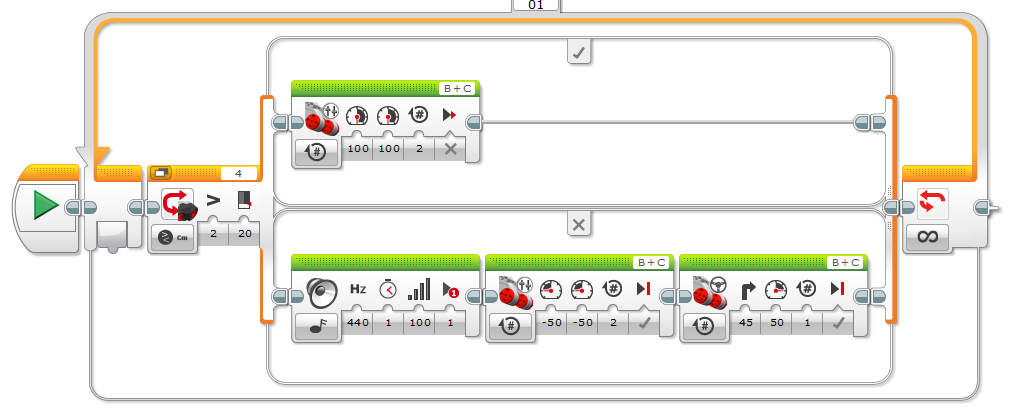
\includegraphics[width= 15cm]{Prog_Ultraschallsensor}
\caption{Lego-Programm zum Test und Kennenlernen des Ultraschallsensor}
\label{fig:ultraschallsensorprog}
\end{figure}
Im der Abbildung \vref{fig:ultraschallsensorprog} wird das, mit der Lego-Programmierumgebung erstellte, Programm dargestellt.\\
Das Programm besteht aus zwei ineinander geschachtelte Schleifen. Die äußere Schleife besitzt keine Abbruchbedingung. Die innere der beiden Schleifen überwacht den Ultraschallsensor und entscheidet je nach Ergebnis des Sensors, was der Roboter machen soll.\\
Trifft der Vergleich \textbf{Vergleich erläutern} zu so fährt der Roboter mit Höchstgeschwindigkeit nach vorne, solange bis sich jedes der Räder genau zweimal gedreht hat. Danach wird auf Grund der Endlosschleife wieder der Ultraschallsensor abgefragt. Diesen Zweig erkennt man an dem Haken über den Anweisungen.

Trifft der Vergleich nicht zu, wird zuerst ein Ton über den integrierten Lautsprecher ausgegeben. Dieser Ton ist ein 440Hz Ton und wird mit voller Lautstärke eine Sekunde lang ausgegeben. Anschliesend fährt der Roboter mit halber Kraft zwei Radumdrehung zurück. Ist dies erledigt, soll sich der Roboter um 45 Grad drehen. Aufgrund der Endlosschleife wird wieder von Vorne begonnen und der Ultraschallsensor wird abgefragt. Dieser Zweig ist in der Darstellung \vref{fig:ultraschallsensorprog} an dem darüber stehenden x zuerkennen.

\section{Testprogramm des Farbsensor}
\begin{figure}[htb]
\centering
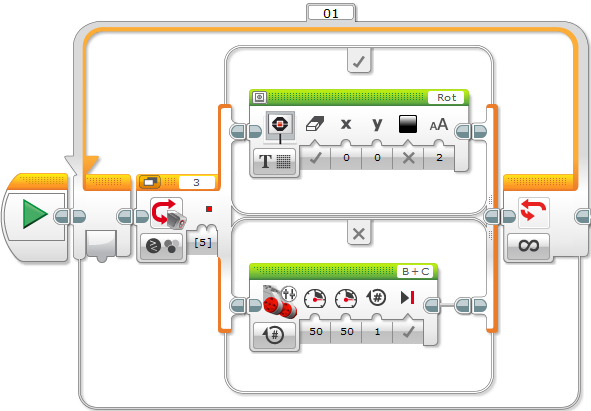
\includegraphics[width= 14cm]{Prog_LichtsensorLego_v1}
\caption{Lego-Programm zum Test und Kennenlernen des Lichtsensors von Lego}
%\label{fig:ultraschallsensorprog}
\end{figure}


